
In this section we present \pisodm, an MDD-based method for building service compositions with non-functional requirements.
Our work provides meta-models for modeling functional and non-functional requirements organized in three levels (Figure~\ref{fig:piSOD-M}): CIM (\textit{Computational Independent Models}), PIM (\textit{Plat\-form Independent Models}) and PSM (\textit{Platform Specific Models}).
Given  high-level models specified at the CIM level, \pisodm proposes the semi-automatic refinement of these models, for the generation of a set of models at the other levels of abstraction.
The refinement process is driven by transformation rules specified between the meta-models.

In the next subsections we present the me\-ta-models from higher to lower levels of abstraction.
The presentation is exemplified by a running example.
The transformations between models are presented in section~\ref{sec:mmrules}.

\begin{figure*}
\centering
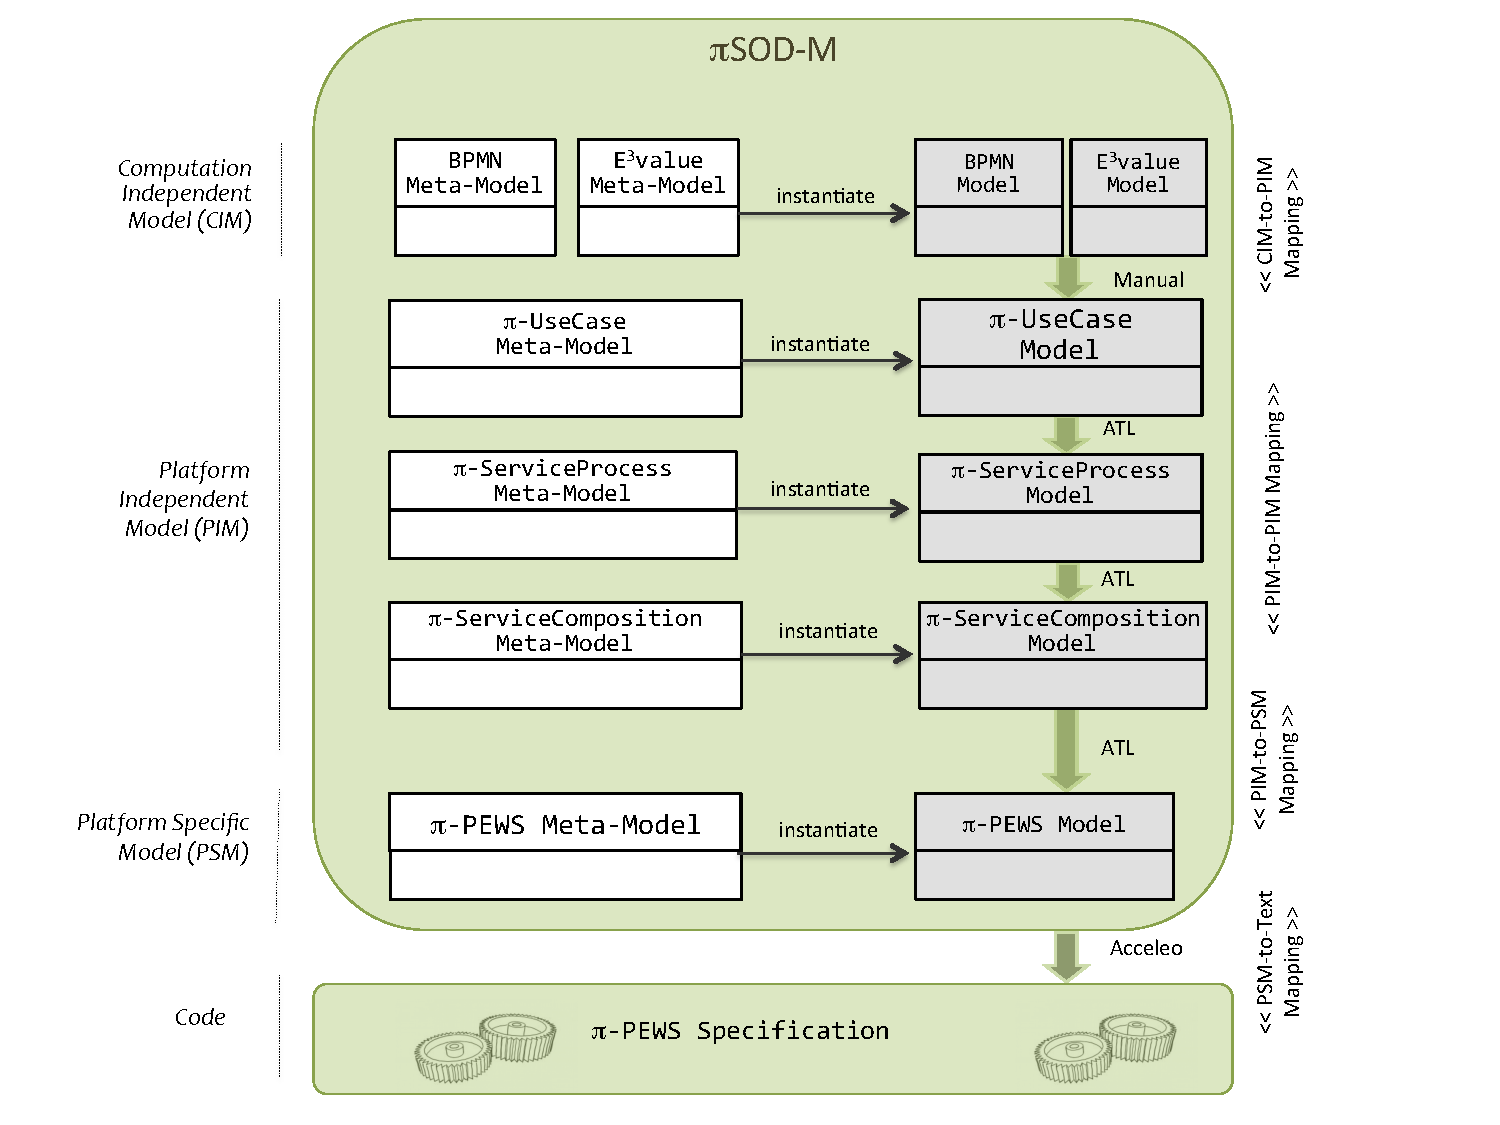
\includegraphics[width=1.0\textwidth]{figs/piSOD-M_process.pdf}
\caption{\pisodm Overview.}
\label{fig:piSOD-M}
\end{figure*}



%. . - -. . - -. . - -. . - -. . - -. . - -. . - -. . - -. . - -. . - -. . - -. . - -. . - -. . - -. . - -. . - -. . - -. . - -. . - -. . - -. . - -. . - -. . - -. . - -. . - -. . - -
\subsection{Computation Independent Models}
%. . - -. . - -. . - -. . - -. . - -. . - -. . - -. . - -. . - -. . - -. . - -. . - -. . - -. . - -. . - -. . - -. . - -. . - -. . - -. . - -. . - -. . - -. . - -. . - -. . - -. . - -

This level focuses on the highest-level view of the system, including its business and requirement specifications.
At this stage of the development, the structure and system processing details are still unknown or undetermined.
\pisodm uses the \textit{e$^3$value}~\cite{Gordijn02valuebased} and \textit{BPMN}~\cite{BPMN} meta-models for this purpose.

% .   .  .   .  .   .  .   .  .   .  .   .  .   .  .   .  .   .  .   .  .   .  .   .  .   .  .   .  .   .  .   .  .   .  .   .  .   .  .   .  .   .  .   .  .   .  .   .  .   .  .   .  .   .  .   .  .   .
\subsubsection{E$^3$value meta-model}
% .   .  .   .  .   .  .   .  .   .  .   .  .   .  .   .  .   .  .   .  .   .  .   .  .   .  .   .  .   .  .   .  .   .  .   .  .   .  .   .  .   .  .   .  .   .  .   .  .   .  .   .  .   .  .   .  .   .

The e$^3$value model of an application identifies the value/information exchange between components of the system.
It is a business model that represents a business case graphically as a set of value exchanges\footnote{See Figure~\ref{fig:CIM:tpme3v}.} ($\nabla$ $\triangle$) and value activities (rounded boxes) performed by business actors (squared boxes).
The model is well suited to enhance the understanding of the environment in which an application is being developed.
It defines \textit{dependency paths}, showing the value exchange between providers and end users when they ask for a service.
A dependency path has a direction and consists of a sequence of linked dependency nodes.
It starts with a \textit{start stimulus} node and ends with an \textit{end stimulus} node (see Figure~\ref{fig:CIM:tpme3v}).
Dependency paths may also contain \textsl{OR} and \textsl{AND} elements (both for initiate and join alternative and parallel paths).

\begin{figure*}
\center
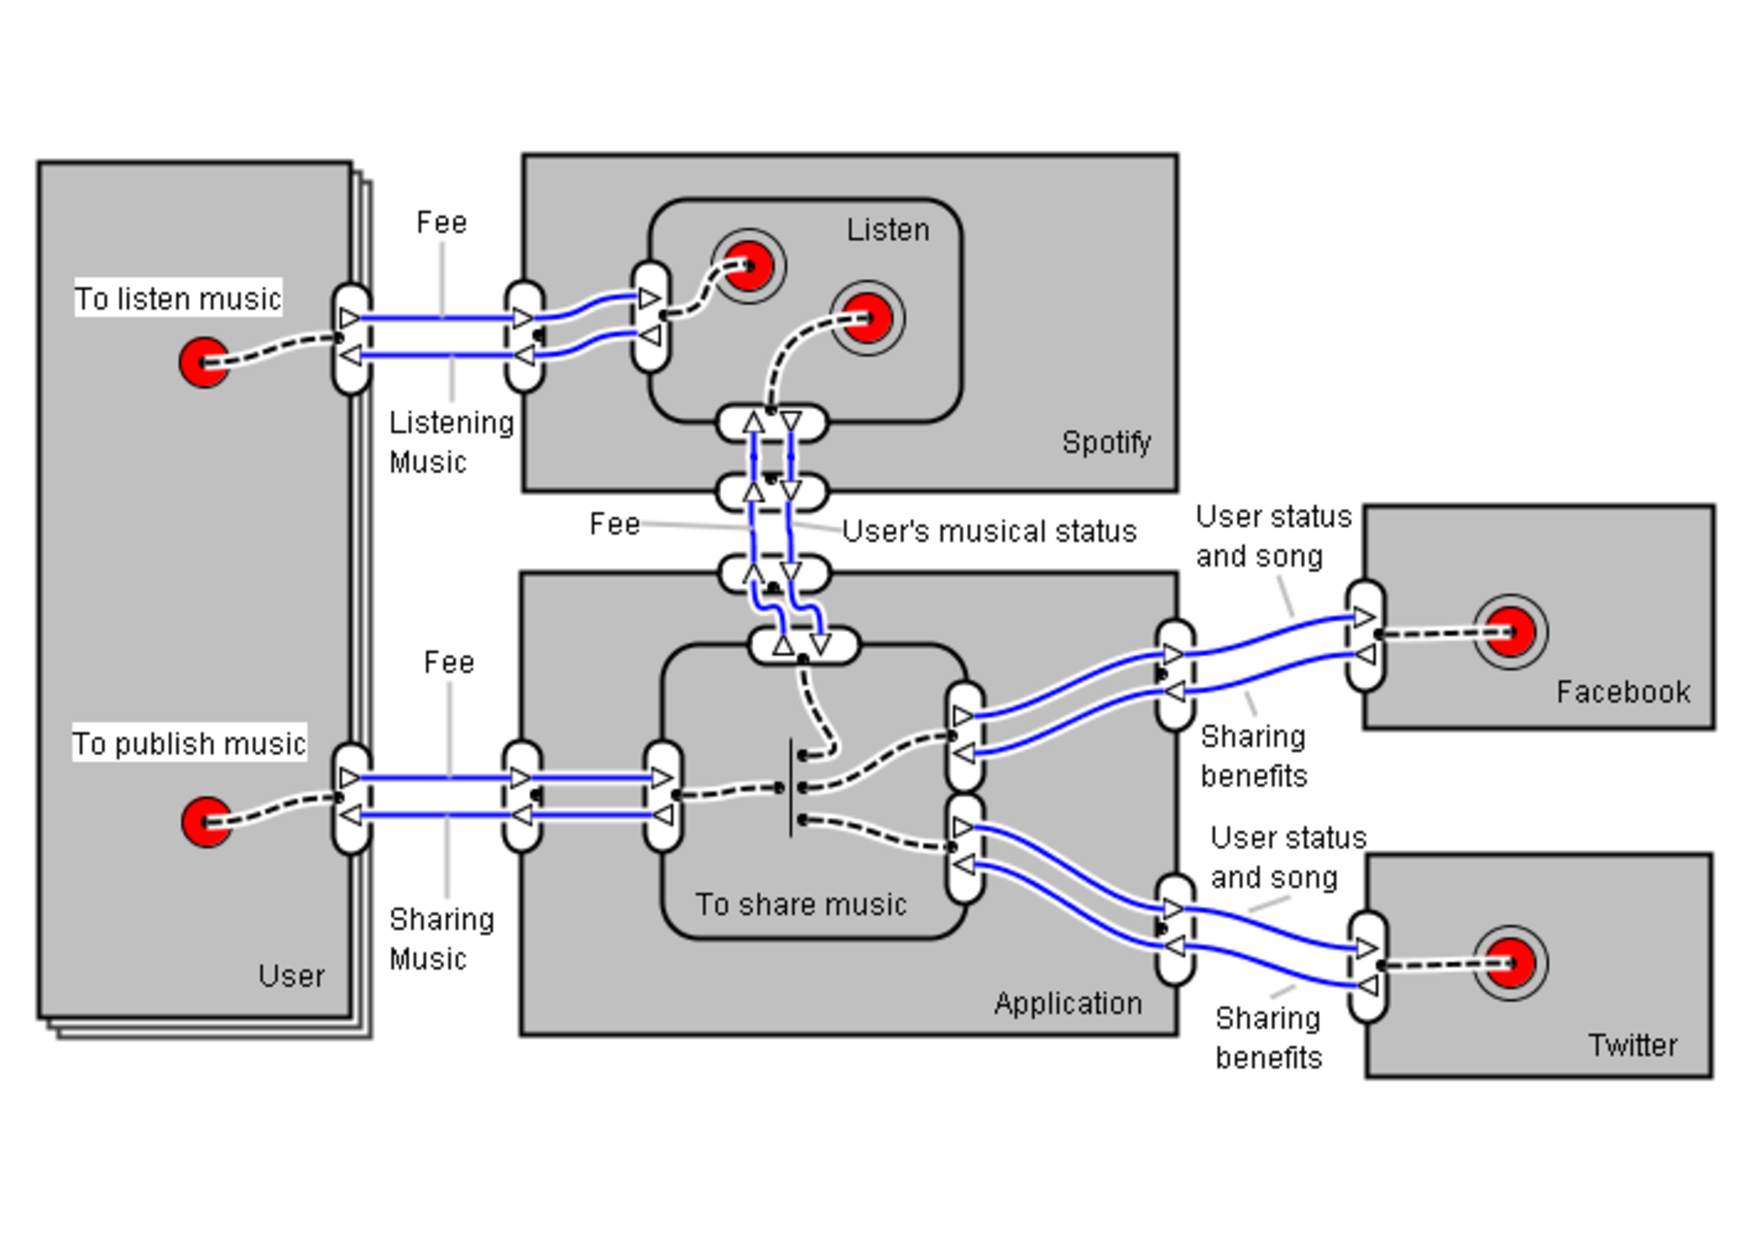
\includegraphics[width=0.75\textwidth]{figs/e3value.pdf}
\hspace*{5cm}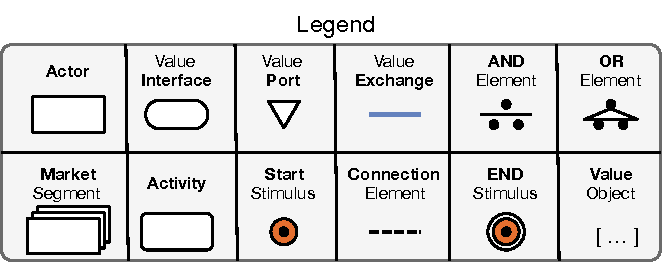
\includegraphics[width=0.4\textwidth]{figs/3ValueKey.pdf}
\caption{\label{fig:CIM:tpme3v} e3value model for ``To Publish Music''.}
\end{figure*}

\begin{example}[To Publish Music]\label{ex:toPublicMusic}
Let us consider the scenario ``To Publish Music'', used as a running example in this section:
An organization wants to provide the service based application ``To Publish Music'' that monitors the music listened by a user during some periods of time and sends the song title  to this person's Twitter and Facebook accounts.
In this way, the user will have her status synchronized in  Twitter and Facebook (i.e., either the same title is published in both accounts or it is not updated) with the title of the music she is listening in Spotify.
The application is based on three external actors ({\em Spotify, Twitter} and {\em Facebook}).
The following (external) services will be used by the application:
\begin{itemize}
\item The  service   Spotify exports a meth\-od for obtaining information  about the music a given user is listening:
\begin{itemize} \item {\sf\small get-Last-Song ( userid ): String} ; \end{itemize}
\item The services Facebook and Twitter export meth\-ods for  updating the status of a given user:
\begin{itemize}
%\item{\sf\small get-Status ( usedid ): String ;
\item {\sf\small update-Status ( userid, new-status ): String};
\end{itemize}
\end{itemize}




The e$^3$value model for ``To Publish Music'' is shown in Figure~\ref{fig:CIM:tpme3v}.
The e$^3$value value model shows Spotify and a private application (which is also a service) that directly interact with users for providing free services for listening and publishing information about music being listened by users. The private application interacts with Spotify for obtaining free information about the flow of music being listened by a user in return of a fee (i.e., premium subscription). Finally, the private application interacts with Facebook and Twitter for updating the user's status.
We can see this interaction as non material benefit sharing (as users subscribe to their networks and are active on them thanks to the private application).
\end{example}

The e$^3$value  model is used to model the (economic) value exchange among the actors involved in an application.
However, the e$^3$val\-ue model does not help to understand the business process of the application nor the conditions in which the different steps of this process are executed.
In order to face this shortcoming, our method proposes the BPMN meta-model as a tool for modelling this aspect of the application.



\subsubsection{BPMN meta-model}

BPMN~\cite{BPMN}  is a graphical representation that establishes the business process of the application through a high-level workflow.
The next example illustrates the use of this meta-model.

\begin{example}[To Publish Music \textit{(cont)}]\label{ex:toPublicMusicBPMN}
Figure \ref{fig:CIM:tpmbpmn} shows the BPMN model\footnote{Details on BPMN (Business Process Management Notation) can be found in http://www.bpmn.org/} of the scenario.
It starts by contacting the music service Spotify for retrieving the user's  musical status (activity {\sf Get Song}).
Twitter and Facebook services are then contacted in parallel for updating the user's status with the corresponding song title (activities {\sf Update Twitter} and {\sf Update Facebook}).
\end{example}
%
\begin{figure}
\center
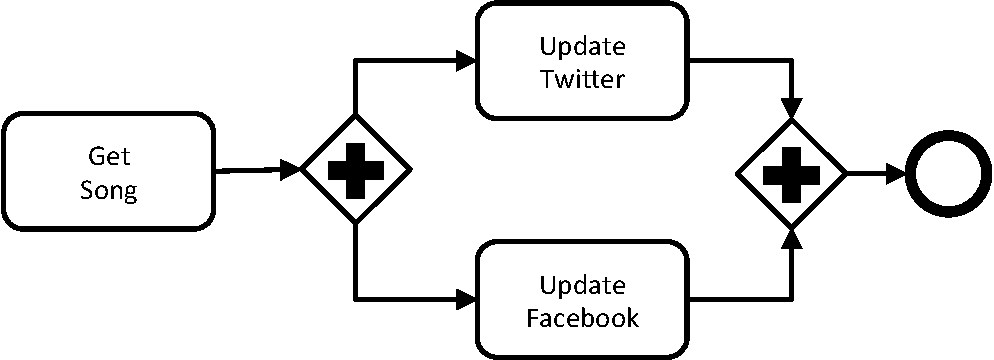
\includegraphics[width=0.45\textwidth]{figs/SC.pdf}
\caption{\label{fig:CIM:tpmbpmn} BPMN model for ``To Publish Music''.}
\end{figure}

The CIM level models are the basis for the development of the application.
The information presented at this level is (manually) refined into PIM-level models of the method \pisodm described next.
Notice that, at this level, the models are (informally) used to describe both functional and non-functional requirements.

%. . - -. . - -. . - -. . - -. . - -. . - -. . - -. . - -. . - -. . - -. . - -. . - -. . - -. . - -. . - -. . - -. . - -. . - -. . - -. . - -. . - -. . - -. . - -. . - -. . - -. . - -
\subsection{Platform Independent Models}
%. . - -. . - -. . - -. . - -. . - -. . - -. . - -. . - -. . - -. . - -. . - -. . - -. . - -. . - -. . - -. . - -. . - -. . - -. . - -. . - -. . - -. . - -. . - -. . - -. . - -. . - -

This level focuses on the system functionality, hiding the details of any particular platform.
The specification defines those parts of the system that do not change from one platform to another.
Our method defines three PIM-level meta-models: \textit{$\pi$-UseCase}, \textit{$\pi$-Ser\-vice\-Pro\-cess} and \textit{$\pi$-ServiceComposition}.

 % .   .  .   .  .   .  .   .  .   .  .   .  .   .  .   .  .   .  .   .  .   .  .   .  .   .  .   .  .   .  .   .  .   .  .   .  .   .  .   .  .   .  .   .  .   .  .   .  .   .  .   .  .   .  .   .  .   .
\subsubsection{\textit{$\pi$-UseCase} meta-model}% .   .  .   .  .   .  .   .  .   .  .   .  .   .  .   .  .   .  .   .  .   .  .   .  .   .  .   .  .   .  .   .  .   .  .   .  .   .  .   .  .   .  .   .  .   .  .   .  .   .  .   .  .   .  .   .  .   .

Figure~\ref{fig:CIM:usecasemetamodel} presents the \textit{$\pi$-UseCase} meta-model.
The goal of \textit{$\pi$-UseCase}  is to be the first representation of the application in terms of functionality, as well as to represent its non-func\-tion\-al requirements.
The notion of \textit{policy} is used to describe NFRs.
(Figure~\ref{fig:CIM:usecasemetamodel} highlights the concepts related to NFRs.)
The \textit{$\pi$-UseCase} meta-model extends the UML Use Case meta-model to describe non-functional requirements with  the following  concepts:  {\sc Business service}, {\sc End consumer}, {\sc Requirement}, {\sc Use Case}, {\sc Composite Use Case}, {\sc Non-\-Func\-tion\-al Requirement}, {\sc Non-Functional} {\sc At\-tri\-bute} and {\sc Constraint}.
An {\sc End Consumer} is represented by an {\sc Actor}.
An  {\sc Actor} is related to {\sc Use Cases} (from the original UML definition), while a {\sc  Composite Use Case} is a set of actions performed by the system which can be broken into different {\sc Use Cases}.
{\sc  Business Service} aggregates several {\sc Use Cases},  a service can be expressed by one or more use cases.
 The {\sc Business Collaborator} concept is represented  through {\sc Packages}.
A {\sc Business Collaborator} represents an external service or a system that interacts with the application that are being modeled.
Each {\sc Business Collaborator} combines the features described in each  {\sc Package}.
%Thus, the services functions can be specified as being grouped into packages.

 \begin{figure*}
\center
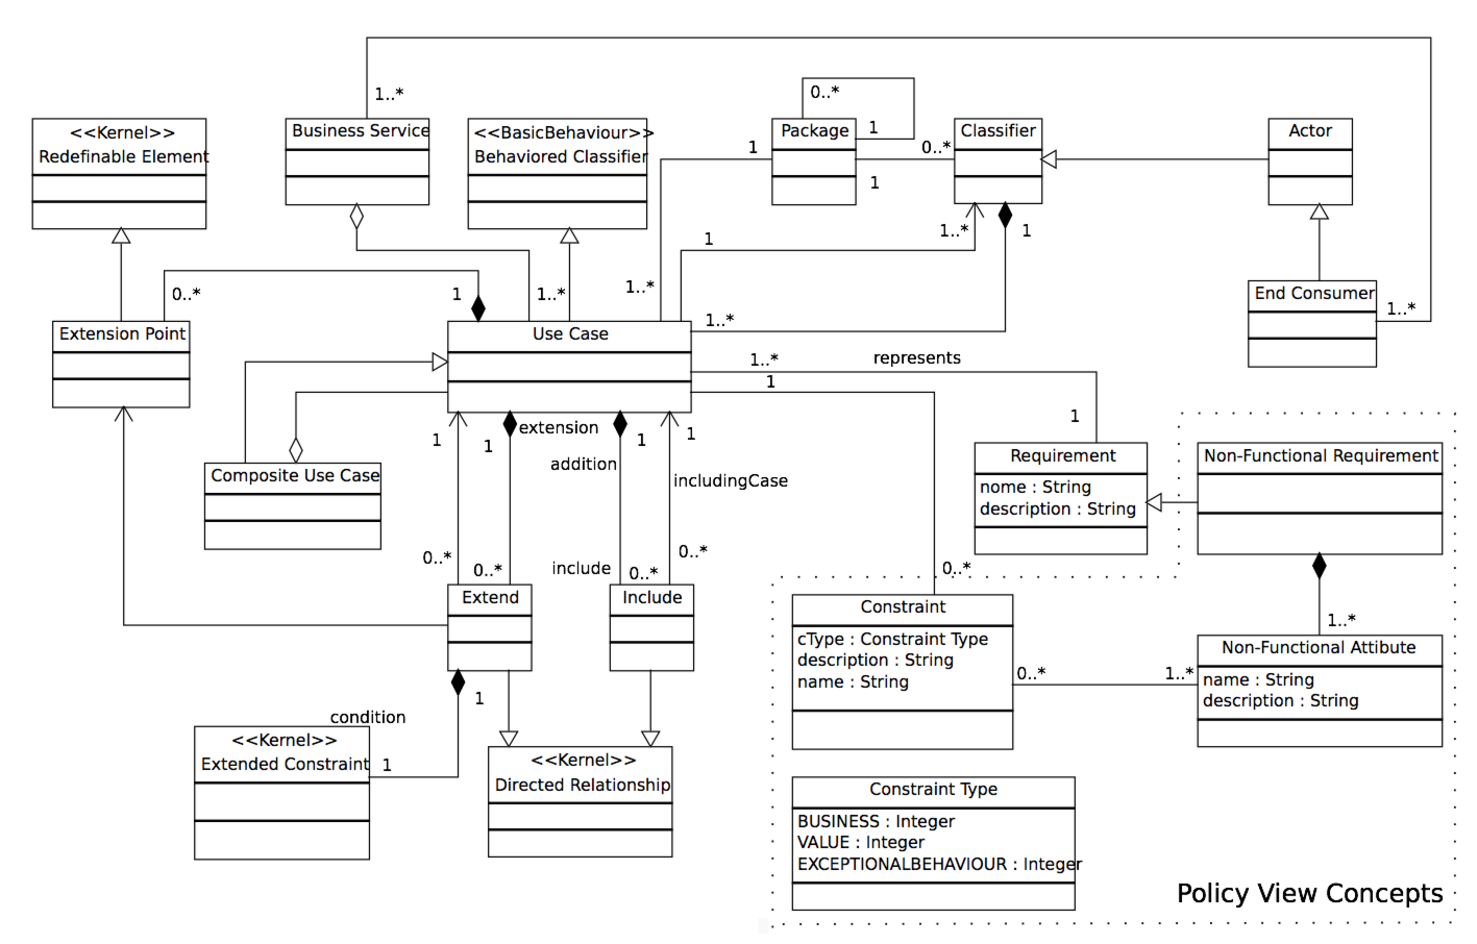
\includegraphics[width=0.9\textwidth]{figs/UseCaseMetaModel.pdf}
\caption{\label{fig:CIM:usecasemetamodel} $\pi$-UseCase Meta-Model.}
\end{figure*}


 The {\sc Non-functional requirement} and {\sc Non-functional Attribute} concepts are represented by {\sc Use Cases} and {\sc Constraints}.
A {\sc Use Case} may have several {\sc Constraints}. Each {\sc Constraint} has a name, description, and a flag to indicate that it has to be  dynamically checked.
Each {\sc Con\-straint} is represented as a stereotyped ({\sf constraint}) use case.
There are three kinds of constraint:
\textit{(i)} A restriction may be associated to data ({\sc Value Constraint}), represented as the stereotype ``value'';
\textit{(ii)} A restriction may correspond to business rules (\textsc{Business Constraint}), represented as the stereotype {\sf ``business''}; and
\textit{(iii)} A restriction may describe {\sc Exceptional Behavior} constraints, represented as the stereotype {\sf ``exceptional\_behavior''}.
The use of these constraints is shown in the following example.

\begin{example}[To Publish Music \textit{(cont)}]\label{ex:toPublicMusic2}
Figure~\ref{fig:CIM:piusecasetpm} shows a $\pi$-UseCase model for our example application.
We consider that, besides the service composition for implementing the application, it is necessary to model  other requirements that represent the (i) conditions imposed by services usage --for example, the fact that both Facebook and Twitter require authentication protocol in order to call their methods for updating the wall; (ii) the conditions stemming from the business rules of the application logic, (e.g., the fact that the walls in Facebook and Twitter must show the same song title and if this is not possible then none of them is updated).

The ``To Publish Music'' Business Service expects  the Facebook or Twitter user status to be changed every time a user starts listening a new song.
Therefore, it is necessary to perform a social network authentication with the users data. Each social network uses different services and different forms of authentication. The authentication constraint is required to update a music status. The restriction is stereotyped as a value constraint, because the users id and password are verified.  Figure \ref{fig:CIM:piusecasetpm} shows the buy music, download music, listen music and pay use cases. The process of buying a song requires the user private data for a Spotify account, and also a secure connection, represented as value and business constraint, respectively. For payment, the user must provide the data of payment card or PayPal account login and password, represented as value stereotype.
Another restriction is that the minimum payment value is 2 euros.
%{\color{red} Talk about this model for the example.}
\end{example}

\begin{figure*}
\center
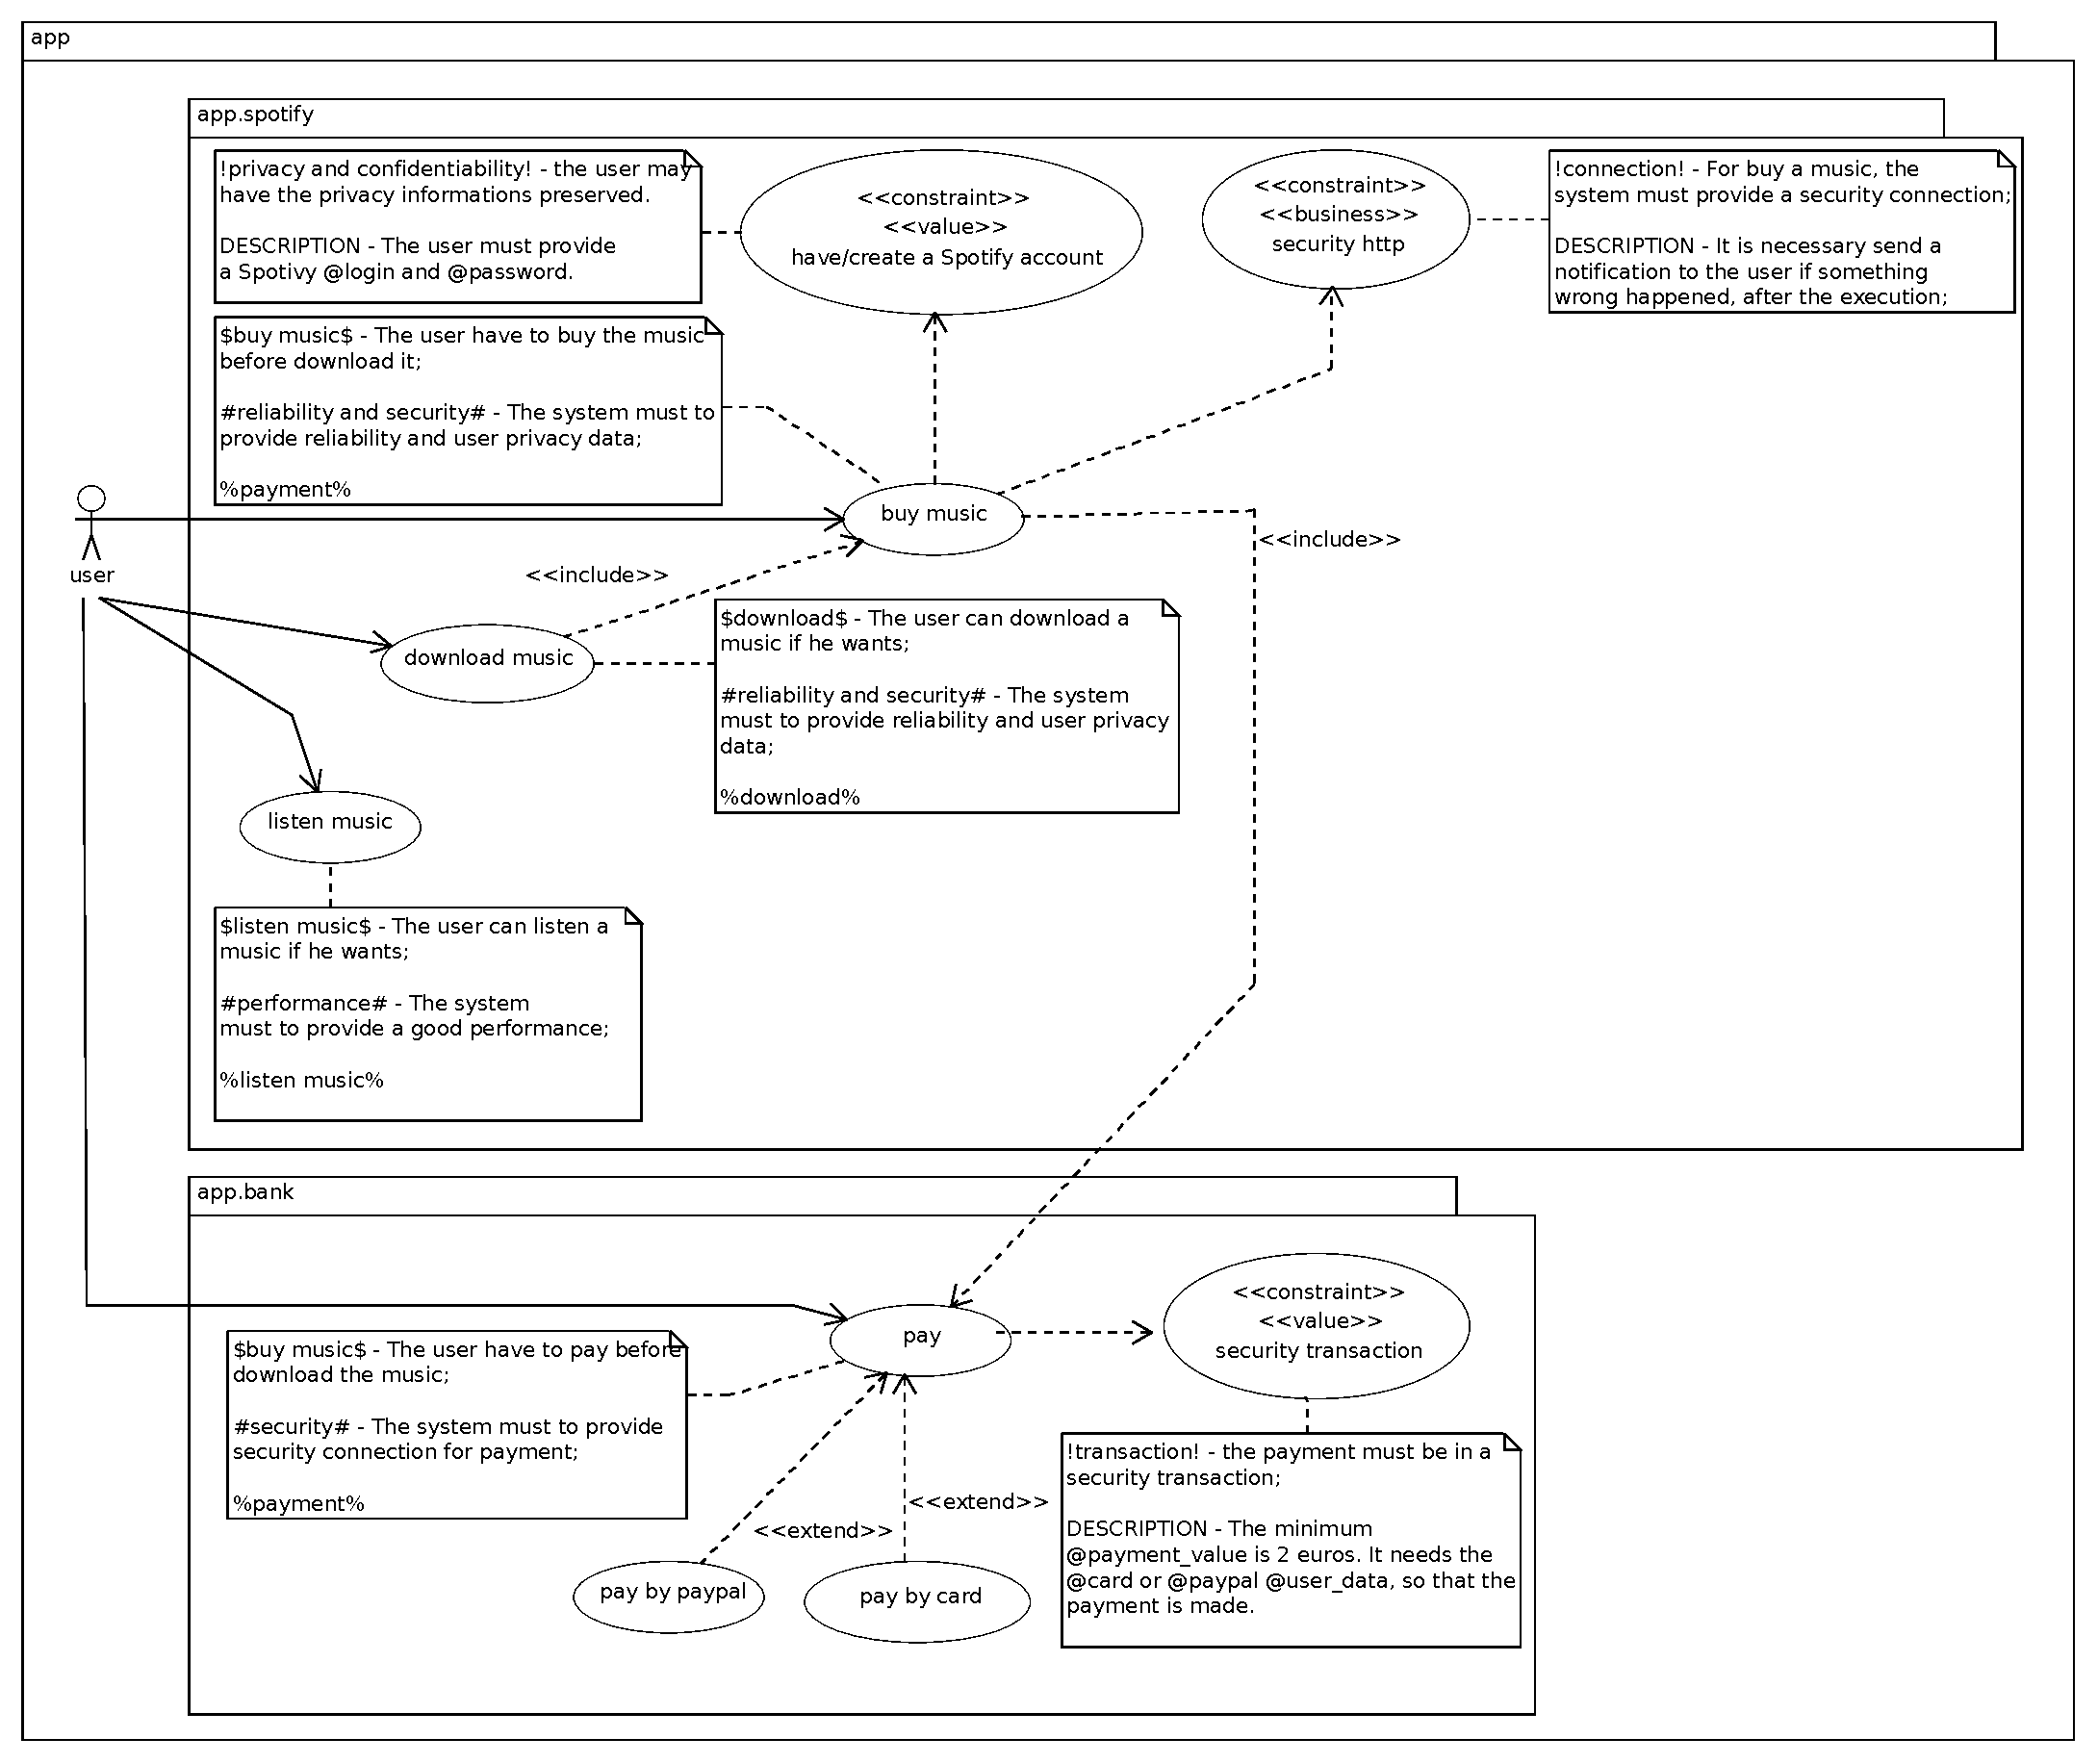
\includegraphics[width=0.9\textwidth]{figs/UseCase.pdf}
\caption{\label{fig:CIM:piusecasetpm} $\pi$-UseCase model for ``To Publish Music''.}
\end{figure*}


 % .   .  .   .  .   .  .   .  .   .  .   .  .   .  .   .  .   .  .   .  .   .  .   .  .   .  .   .  .   .  .   .  .   .  .   .  .   .  .   .  .   .  .   .  .   .  .   .  .   .  .   .  .   .  .   .  .   .
\subsubsection{\textit{$\pi$-ServiceProcess} meta-model}% .   .  .   .  .   .  .   .  .   .  .   .  .   .  .   .  .   .  .   .  .   .  .   .  .   .  .   .  .   .  .   .  .   .  .   .  .   .  .   .  .   .  .   .  .   .  .   .  .   .  .   .  .   .  .   .  .   .

The \textit{$\pi$-ServiceProcess} meta-model extends the UML activity diagram with the concept of \textit{contract} to represent constraints over data and actions. This concept is used to model
groups  of  constraints  in the \textit{$\pi$-UseCase}.
In Figure~\ref{fig:CIM:serviceprocessmetamodel}, the concepts of the \textit{$\pi$-Ser\-vice\-Process} meta-model are: {\sc Contract}, {\sc Assertion}, {\sc Exceptional behavior}, {\sc Activity}, {\sc Ser\-vice Acti\-vi\-ty}, {\sc Action} and {\sc Constraint}.
The dotted part of the figure defines those concepts related to the representation of NFRs.

A specific \textit{$\pi$-ServiceProcess} model shows the set of logically related activities to be performed in a service-based application.
So, the activities of this model represent a behavior that is part of the business logic of the application.
A \textit{$\pi$-ServiceProcess}  model contains three main elements: (i) service process, (ii) service activity and (iii) activity contract. A service activity represents an operation that is part of the execution flow, and it is modeled as an {\sc Action}.
An activity contract represents the {\sc Non-functional Requirement}  that is also part of the execution flow of a service, identified  as a stereotyped activity ({\sf assertion}).
The {\sc Assertion}s associated to an {\sc Action} compose a {\sc Contract}. 
Using the concepts {\sc Contract} and {\sc Assertion} it is possible to specify each activity service, by defining its pre-conditions and post-conditions.

\begin{figure*}
\center
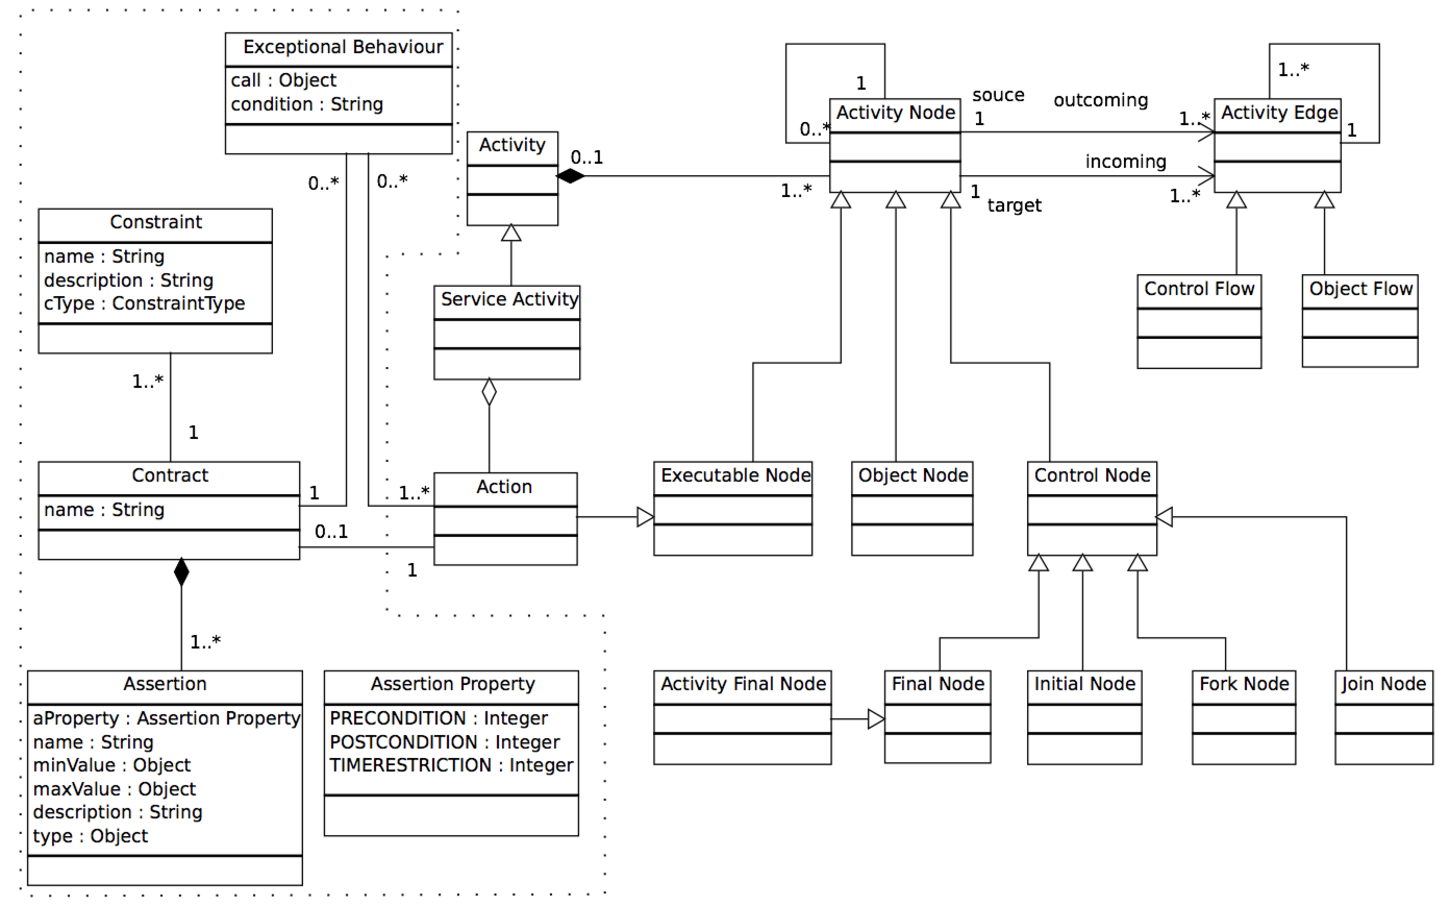
\includegraphics[width=0.9\textwidth]{figs/ServiceProcessMetaModel.pdf}
\caption{\label{fig:CIM:serviceprocessmetamodel} $\pi$-Service Process Meta-Model.}
\end{figure*}

%According to the meta-model, a \textit{$\pi$-ServiceProcess} model represents the service processes and its contracts. It models the set of system activities and describe contracts for each activity or the process as a whole. Each service identified in the previous model (\textit{$\pi$-UseCase}) is mapped to an action. This model defines a workflow for  modeling business logic and the behaviour of the application being developed. The behaviour is represented by each action and the restrictions by the assertion description. All assertions are described by stereotyped actions.

\begin{example}[To Publish Music \textit{(cont)}]\label{ex:toPublicMusic3}
Considering the example scenario, the contract based process of activities  is shown in figure \ref{fig:CIM:serviceprocess}. The buy music and publish music services (update Twitter and Facebook) have pre- and post-conditions assertions that are composed into a contract for each service. The buy music pre-conditions consist in verifying:
(i) if the User data are correct;
(ii) if the User is already logged in Spotify;
(iii) if bank account information are correct and;
(iv) if there are enough funds in the bank account to cover the payment.
A post-condition ensures the complete transaction and verifies if a notification was sent to the user and Spotify, about the payment authorization. There are four assertions for the buy music action, and each assertion has been detailed with the assertion property and predicate that must be verified. To update services, depending of each service, there may be different restrictions. As an example, a new verification of user data and message format is appropriate (maximum 140 characters), in the case of Twitter. In the case of Facebook, it is required that the user is already logged in Spotify and these data are the same as Facebook.
As post-condition, the application ensures that the Facebook service sends a notification of success.
To update Twitter a pre-condition is required, while to update Facebook it is necessary to check a pre-condition and a confirmation notice (modeled as post-condition).
As a pre-condition for ``twitter update'' it is necessary that (i) the music format is correct and (ii) the twitter login and password are correct for the update.
\end{example}

\begin{figure*}
\center
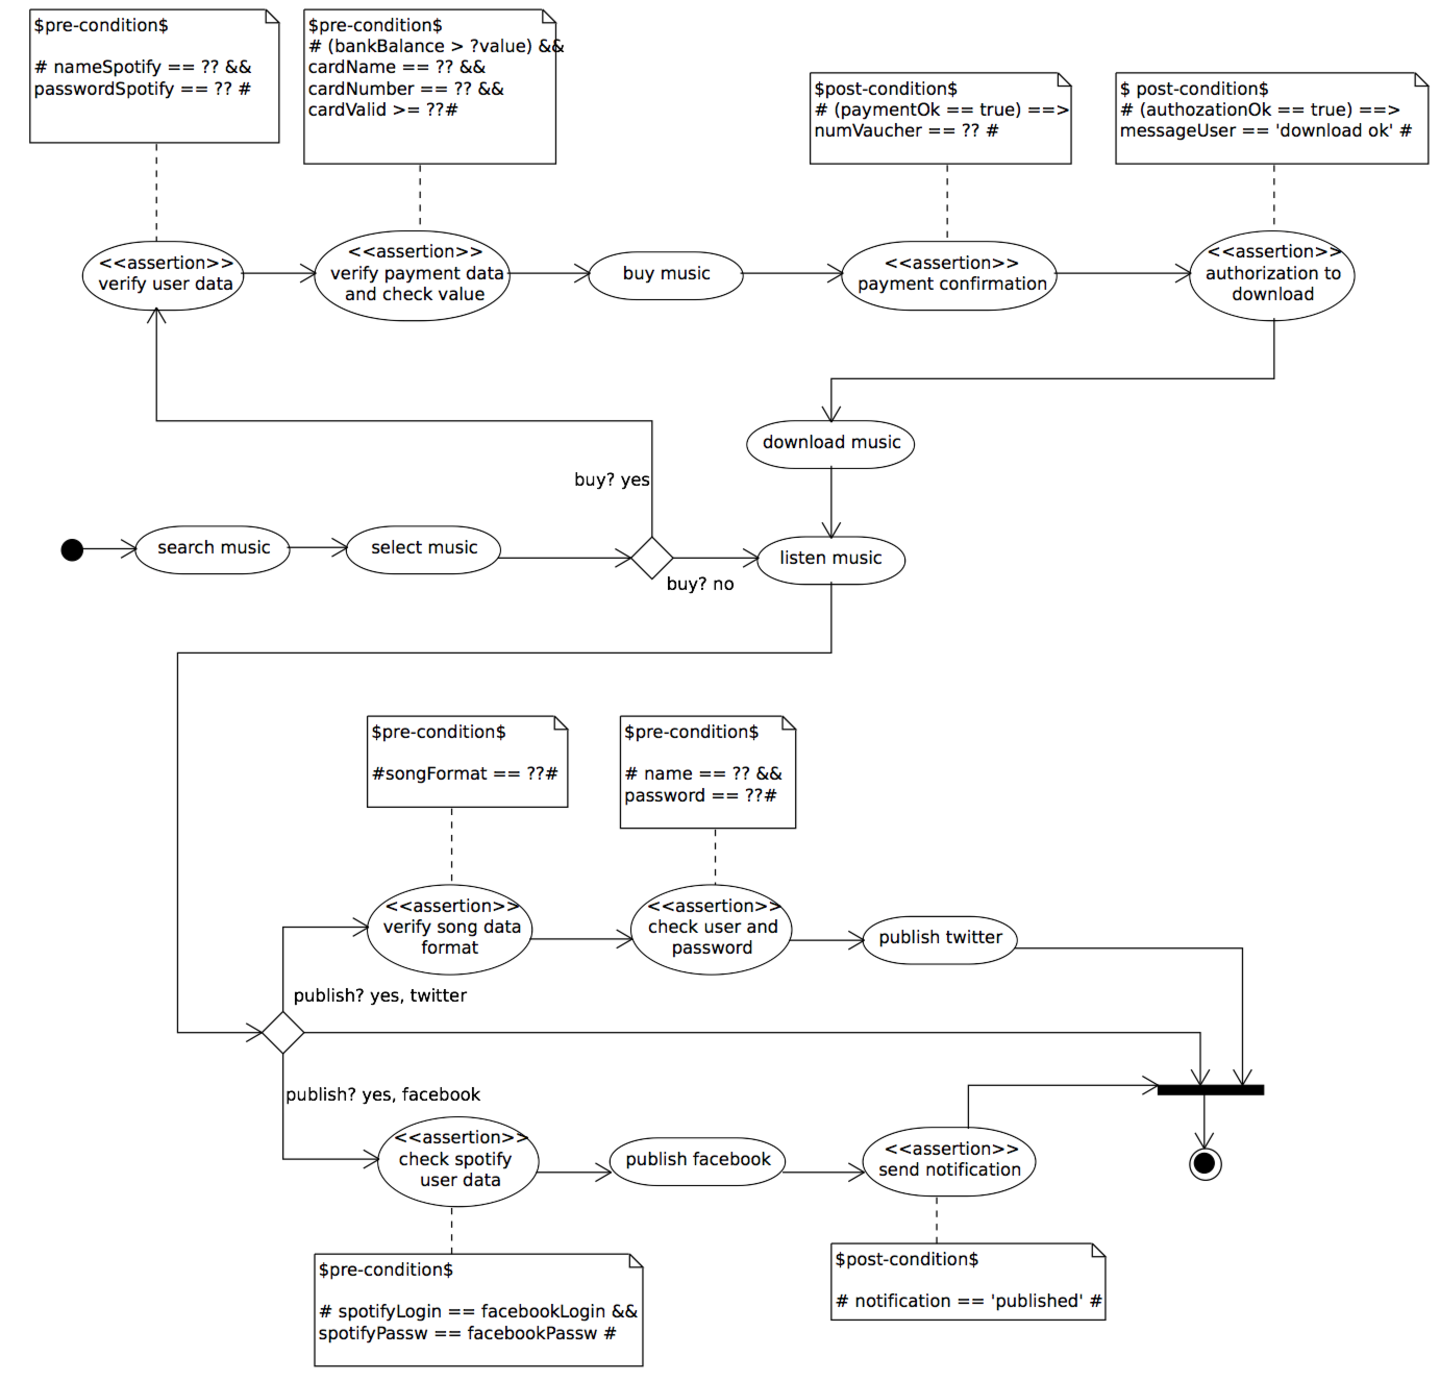
\includegraphics[width=0.9\textwidth]{figs/ServiceProcess.pdf}
\caption{\label{fig:CIM:serviceprocess} $\pi$-ServiceProcess model for ``To Publish Music''.}
\end{figure*}

% .   .  .   .  .   .  .   .  .   .  .   .  .   .  .   .  .   .  .   .  .   .  .   .  .   .  .   .  .   .  .   .  .   .  .   .  .   .  .   .  .   .  .   .  .   .  .   .  .   .  .   .  .   .  .   .  .   .
\subsubsection{\textit{$\pi$-ServiceComposition} meta-model}% .   .  .   .  .   .  .   .  .   .  .   .  .   .  .   .  .   .  .   .  .   .  .   .  .   .  .   .  .   .  .   .  .   .  .   .  .   .  .   .  .   .  .   .  .   .  .   .  .   .  .   .  .   .  .   .  .   .

In Figure \ref{fig:e-scomposition-metamodel}, the $\pi$-Serv\-ice\-Com\-po\-si\-tion meta-model
provides meta-classes to represent workflows\footnote{Workflows are transformed into implemented service compositions.} that model  business processes.
The \textit{$\pi$-Serv\-ice\-Com\-po\-si\-tion} meta-model extends the UML activity  meta-model with the concept of  \textit{A-Policy}
to group contracts with similar non-functional requirements.
For instance, security and privacy restrictions may be grouped into a security policy.
 The  ($\pi$-Serv\-ice\-Com\-po\-si\-tion) meta-model defines:
%In the meta-model of Figure~\ref{fig:e-scomposition-metamodel}:
\begin{itemizedTrivlist}
\item A {\sc Business Collaborator} meta-class, to represent the classes of entities that collaborate in  business processes by performing some  required action.
An instance of this meta-class is graphically represented as a partition in the activity diagram.
A collaborator can be either internal or external to the system.
When the collaborator of the business is external to the system, the attribute {\sf IsExternal}\footnote{We use the {\sf sans serif} font for referring to classes defined using a meta-model.} of the collaborator is set to \textbf{true}.

\item {\sc Action}s, a kind of {\sc ExecutableNode}, are represented in the model as a class activity instance of the meta-class \textsc{Action}.
A class action represents some type of transformation or processing.
There are two types of actions: i) a WebService (attribute Type is {\sf WS}); and ii) a simple operation called an {\sc ActivityOperation} (attribute Type is {\sc AOP}).

\begin{figure*}
\centering
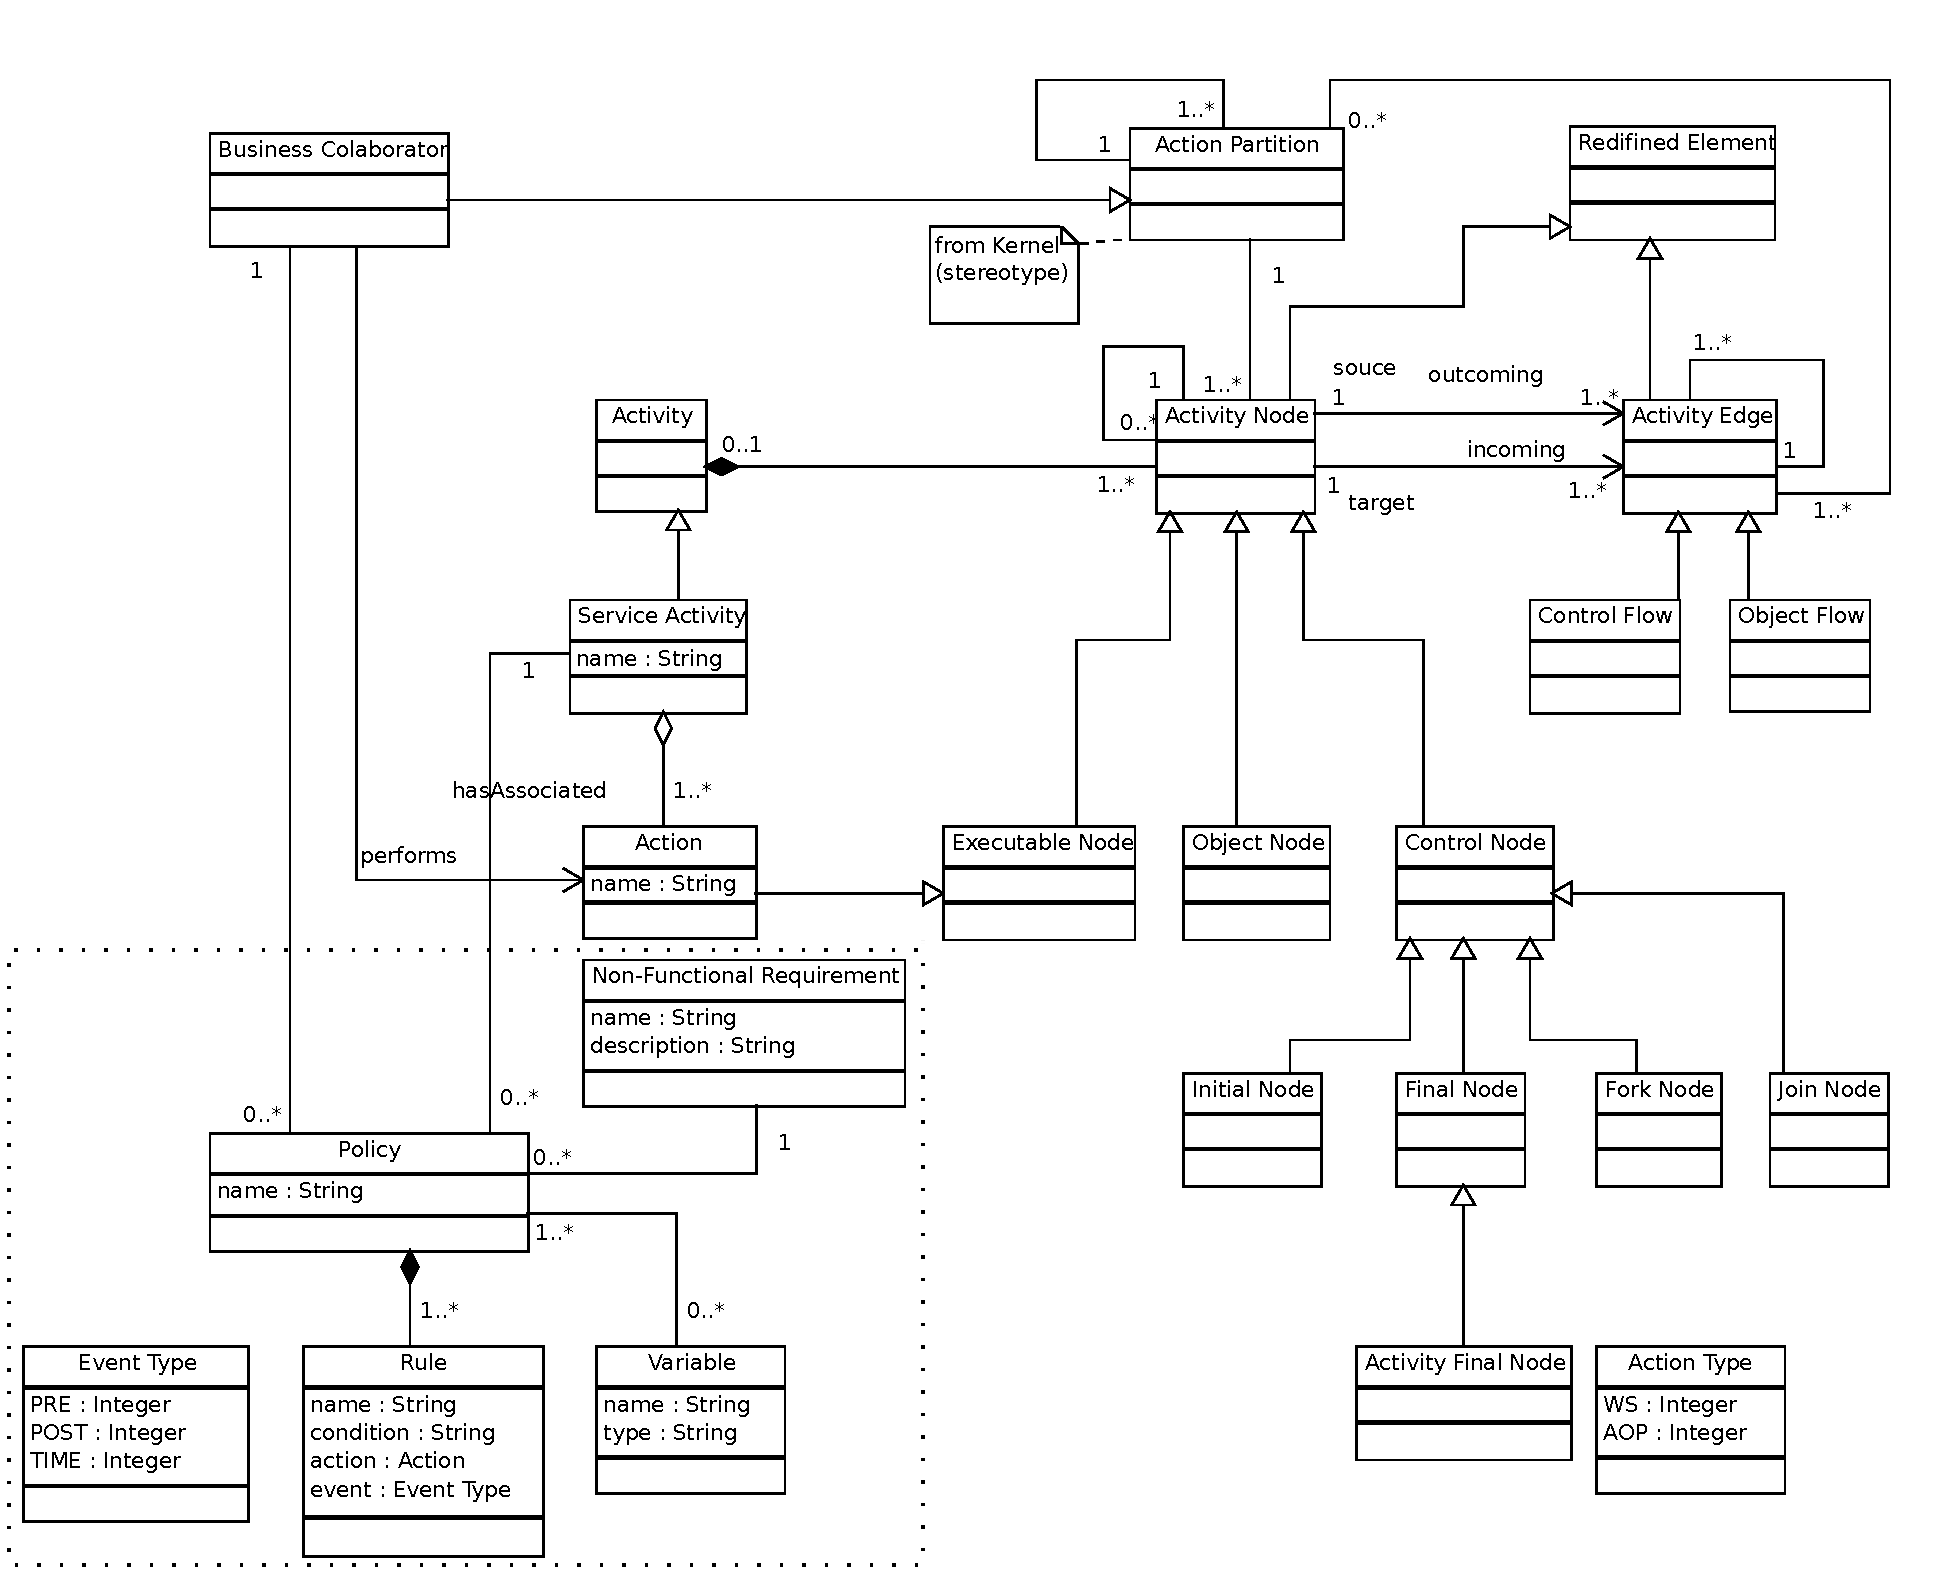
\includegraphics[width=1.0\textwidth]{figs/PiServiceComposition}
\caption{$\pi$-Service Composition Meta-model.}
\label{fig:e-scomposition-metamodel}
\end{figure*}

\item The {\sc ServiceActivity} meta-class represents classes of composite activity types that must be carried out as part of a business service and is composed by one or more execu\-ta\-ble nodes.

\item In order to represent constraint types associated to services compositions, we defined the me\-ta- classes {\sc Rule} and {\sc A-policy} (see blue meta-classes in the $\pi$-Serv\-ice\-Com\-po\-si\-tion meta-model in Figure \ref{fig:e-scomposition-metamodel}).
We model non-func\-tion\-al constraints by using the notion of {\em A-policy}~\cite{Espinosa-Oviedo2011a,CIC:eovszmc09c}.
An {\em A-policy} is defined by attributes and rules.
The conditions of each rule are evaluated.
In case of failure, the actions of the rule will be performed.
The meta-class {\sc Rule} represents event-condition-action rules where the {\sc Event} part represents the moment in which a constraint  is evaluated.
An {\em A-policy} defines variables and operations that can be shared by the rules and that can be used for expressing their Event and Condition parts.
\end{itemizedTrivlist}
Instances of this meta-model are represented as UML activity diagrams.
\begin{figure*}
\centering
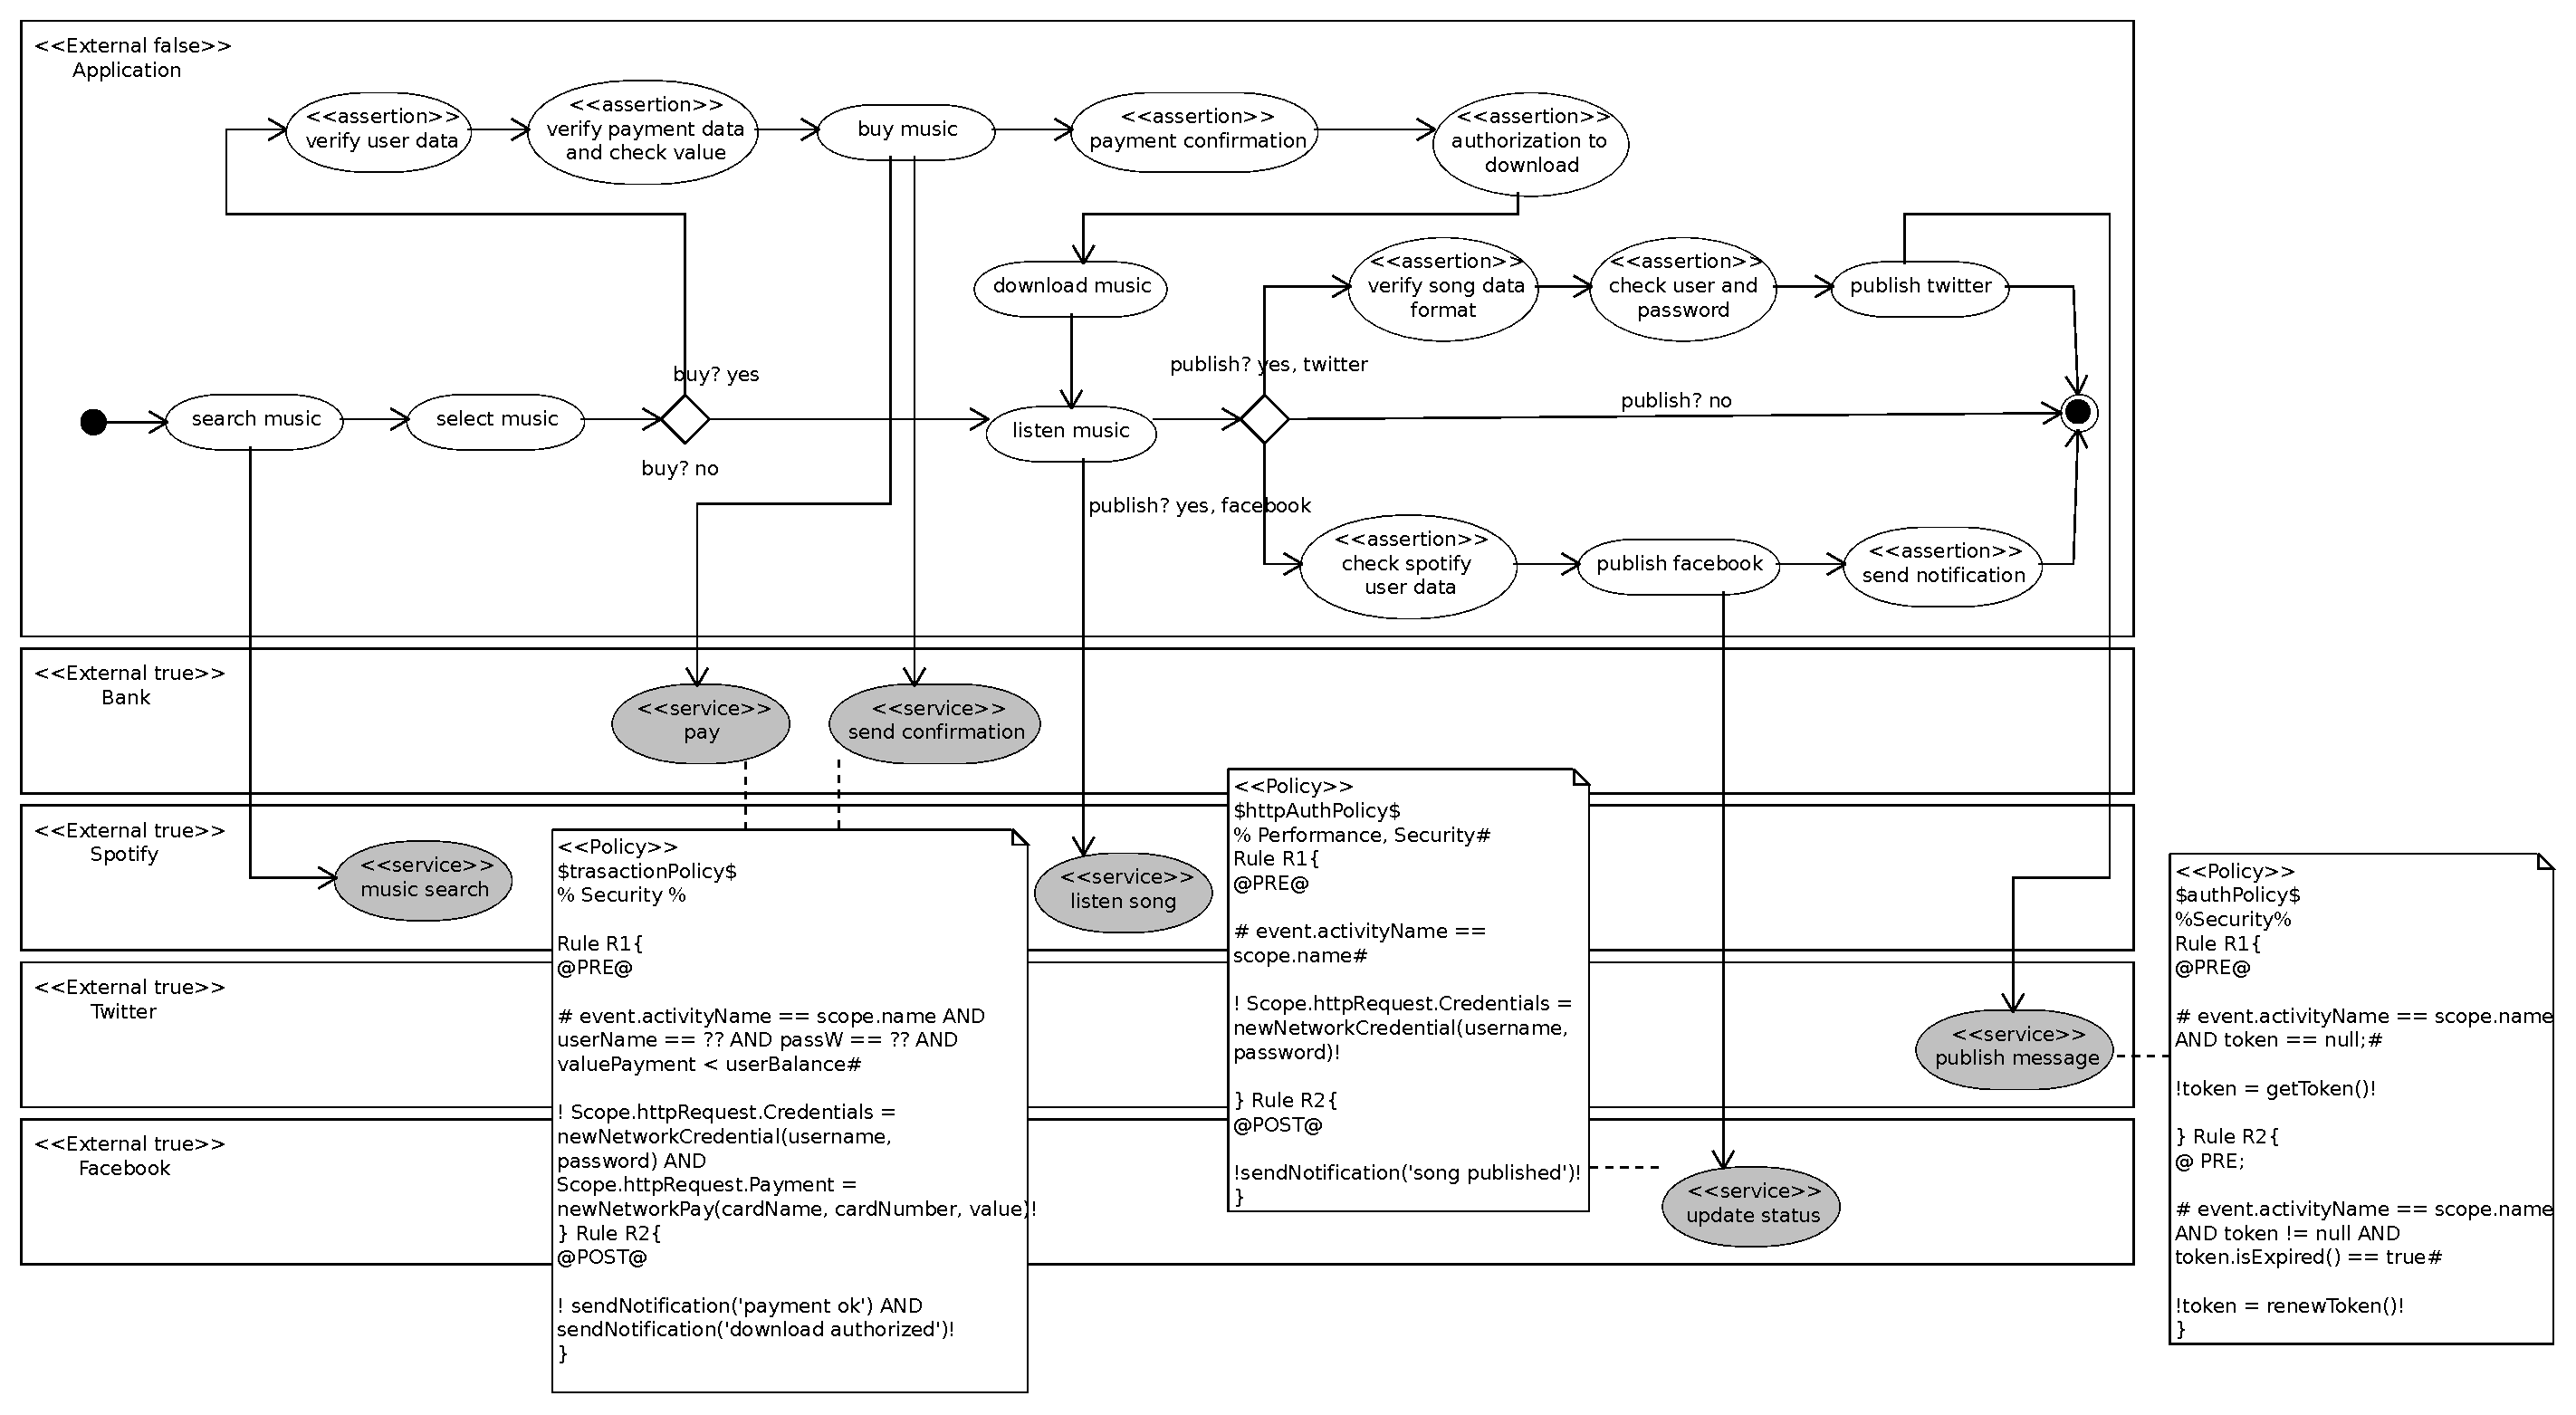
\includegraphics[width=0.95\textwidth]{figs/piServiceComposition-toPublishMusic}
%{\color{red}\LARGE PLACIDO: Please change the names of the boxes in accordance to the explanation --Martin}
\caption{$\pi$-ServiceComposition Model for the ``To publish
music'' business service.}
\label{fig:servicecompositionmodel}
\end{figure*}

\begin{example}[To Publish Music \textit{(cont)}]\label{ex:toPublicMusic4}
To illustrate the use of the $\pi$-Service Composition meta-model, we define a model for the ``To Publish Music'' scenario (Figure \ref{fig:servicecompositionmodel}).
 We model a business process with three service activities: {\em Listen Music}, {\em Publish Music} and {\em Confirmation}.
The {\em Publish Music} activity calls the {\em Facebook} and {\em Twitter} services.
Both {\em Facebook} and {\em Twitter} require authentication.
Two authentication policies are required, one for {\em Twitter} and another for {\em Facebook}.
%{\color{red} To be completed!.}
In this model, there are three external business collaborators ({\em Spotify, Twitter} and {\em Facebook}).
% \footnote{We use {\em italics} to refer to concrete values of the classes of a model that are derived from the classes of a meta-model.}).
The model also shows the business process of the application that consists of three service activities: {\em Listen Music}, {\em Publish Music} and {\em Confirmation}.
Note that  the activity {\em Publish Music} calls the actions of two service collaborators namely {\em Facebook} and {\em Twitter}.
Both {\em Facebook} and {\em Twitter} services require authentication protocols in order to execute methods that read and update the user data.
%A call to such services must be part of the authentication protocol required by these services.
In the example, we  associate two authentication policies, one for the open authentication protocol, represented by the class {\sf\small OAuthPolicy} at {\em Twitter}, associated to the activity  {\sf\small UpdateTwitter} (see Figure \ref{fig:servicecompositionmodel}).
In the same way, the {\em Facebook} class {\sf\small HTTPAuthPolicy}, for the http authentication protocol is associated to the activity {\sf\small UpdateFacebook}.
{\sf\small OAuthPolicy} implements the open authentication protocol.
The {\em A-policy} {\sf\small OAuthPolicy} has a variable {\sf\small Token}, used to store the authentication token provided by the service.
This variable is imported through the library {\sf\small OAuthPolicy.Token}.
The A-policy {\sf\small OAuthPolicy} defines two rules, both can be triggered by events of type {\sf\small ActivityPrepared}: (R$_1$): If no token has been associated to the variable {\sf\small token}, then a token is obtained ; and (R$_2$): if the token has expired, then it is renewed.
Notice that the code in the actions profits from the imported {\sf\small OAuthPolicy.Token} for transparently obtaining or renewing a token from a third party.
{\sf\small HTTPAuthPolicy} implements the HTTP-Auth protocol.
The A-policy imports an http protocol library and it has two variables {\sf\small username} and {\sf\small password}.
The event of type {\sf\small ActivityPrepared} is the triggering event of the rule {\sf\small R$_1$}.
On the notification of an event of that type, a credential is obtained using the username and password.
\end{example}

%We propose the use of rules and policies to model and associate non-functional properties to service compositions.
%These artifacts will be used to generate the actual programs that will implement the application:
Once the $\pi$-Service Composition Model has been defined, then it can be transformed into a lower level model (in our case, $\pi$-PEWS) that gives support to code generation.
The $\pi$-PEWS  meta-model is described in the next section.


%. . - -. . - -. . - -. . - -. . - -. . - -. . - -. . - -. . - -. . - -. . - -. . - -. . - -. . - -. . - -. . - -. . - -. . - -. . - -. . - -. . - -. . - -. . - -. . - -. . - -. . - -
\subsection{Platform Specific Models}
%. . - -. . - -. . - -. . - -. . - -. . - -. . - -. . - -. . - -. . - -. . - -. . - -. . - -. . - -. . - -. . - -. . - -. . - -. . - -. . - -. . - -. . - -. . - -. . - -. . - -. . - -

This level focuses on the functionality, in the context of a particular implementation platform.
Models at this level put together the platform-independent view with the specific aspects of the platform to implement the system.
Models at the PSM level can be automatically translated into actual computer programs.
We have defined one meta-model at this level.

\textit{$\pi$-PEWS} provides con\-cepts for modelling service compositions.
Instances of this meta-model are textual descriptions of service compositions that can be translated into any service composition language, such as BPEL~\cite{bpel03} or PEWS~\cite{BaCAM05,Placido2010LTPD}.

PEWS~\cite{BHM06,Placido2010LTPD} is a notation to express service compositions.
The language is based on the notion of Path Expressions~\cite{And79} and can easily be translated into any actual composition language, such as BPEL~\cite{bpel03}.
Figure~\ref{fig:PPEWSmetamodel} presents the $\pi$-{\sc Pews} meta-model, where we identify classes to describe:
\begin{itemizedTrivlist}
\item Service compositions: {\sc Namespace} representing the interface exported by a service, {\sc Operation} that represents a call to a service method, {\sc CompositeOperation}, {\sc Operator} and {\sc Path} for representing service compositions.
A {\sc Path} can be an {\sc Operation} or a {\sc Compound Operation}.
A {\sc Compound Operation} is defined using an {\sc Operator}.
The language defines operators to denote guarded operations ($[C]S$); sequential ($\ . \ $), parallel ($\ \| \ $) and alternative ($\ + \ $) compositions; as well as sequential ($*$) repetition.

\item {\em A-Policies} that can be associated to a service compositions:  {\sc A-Policy}, {\sc Rule}, {\sc Event}, {\sc Condition}, {\sc Action}, {\sc State}, and {\sc Scope}.
A brief description of these classes is given next.
\end{itemizedTrivlist}
%
\begin{figure*}
\centering
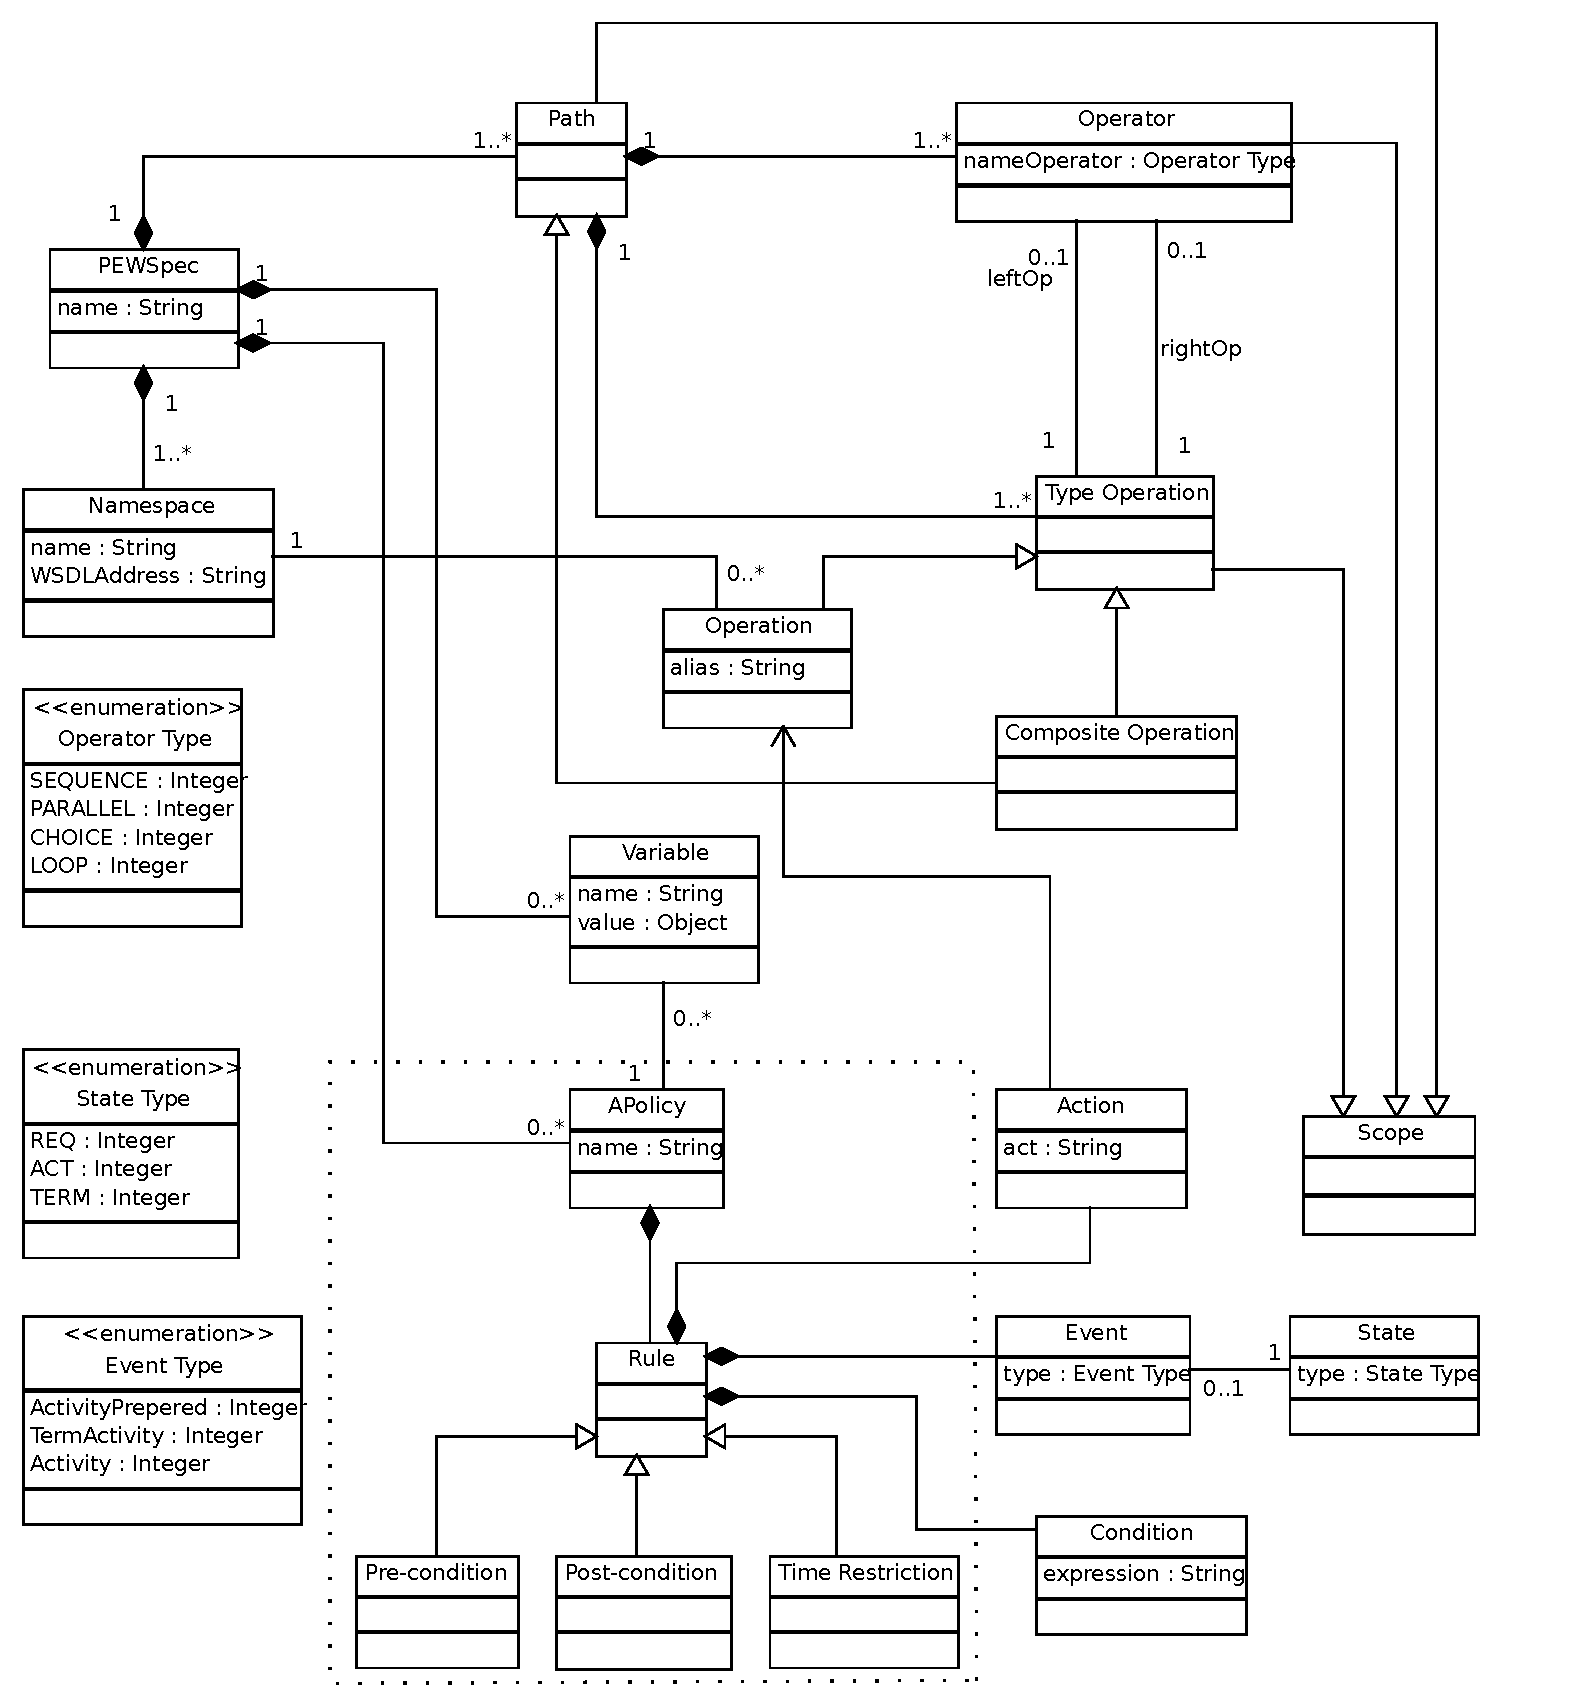
\includegraphics[width=0.75\textwidth]{figs/PEWSMetamodel}
\caption{$\pi$-{\sc Pews} Meta-model.}
\label{fig:PPEWSmetamodel}
\end{figure*}

Figure~\ref{fig:PPEWSmetamodel} shows that each {\sc A-Policy} is associated to a {\sc Scope} that can be either an {\sc Operation} (e.g., an authentication protocol associated to a method exported by a service),  an {\sc Operator} (e.g., a temporal constraint associated to a sequence of operators) or a {\sc Path}.
Each {\sc A-Policy} groups a set of ECA rules with a classic semantics, i.e, {\em when an event of type E occurs, if condition C is verified then execute the action A}.
In this way, an {\em A-policy} represents a set of reactions to be possibly executed when one or several events are notified.


\begin{example}[To Publish Music \textit{(cont)}]\label{ex:toPublicMusic5}
Figure \ref{fig:Specific-Contract-Representation} shows the $\pi$-PEWS code resulting from the $\pi$-service composition model of our scenario example.
Notice that the code contains namespaces and definitions (obtained by using information about the business collaborators of the $\pi$-SCM model), a workflow expression \textit{(Path)} containing operation calls and contracts (derived from the \textit{A-Policies}).
\end{example}

\begin{figure*}
\centering

\includegraphics[width=0.8\textwidth]{figs/pi-pewsSpecification-toPublishMusic}
\caption{$\pi$-PEWS Specific and Policy Representation.}
\label{fig:Specific-Contract-Representation}
\end{figure*}

